\documentclass[11pt, a4paper]{article}

%%%%%%%%%%%%%%%%%
% Configuration %
%%%%%%%%%%%%%%%%%
\usepackage{allrunes}
\usepackage{amsmath}
% If magyar is wanted
% \usepackage[magyar]{babel}
\usepackage[T1]{fontenc}
\usepackage[utf8]{inputenc}
\usepackage{fixltx2e}
\usepackage{multirow}
\usepackage{url}
\usepackage{amsfonts}
\usepackage{amsthm}
\usepackage{mathtools}
\usepackage{amssymb}
\usepackage{xcolor}

% feynman diagrams
\usepackage{tikz-feynman}

% using circled symbols
\usepackage{tikz}
\newcommand*\circled[1]{\tikz[baseline=(char.base)]{
            \node[shape=circle,draw,inner sep=2pt] (char) {#1}}}


% Here you can configure the layout
\usepackage{geometry}
\geometry{top=1cm, bottom=1cm, left=1.25cm,right=1.25cm, includehead, includefoot}
\setlength{\columnsep}{7mm} % Column separation width

\usepackage{graphicx}

%\usepackage{gensymb}
\usepackage{float}

% For bra-ket notation
\usepackage{braket}

% To have a good appendix
\usepackage[toc,page]{appendix}

\usepackage{abstract}
\renewcommand{\abstractnamefont}{\normalfont\bfseries}
\renewcommand{\abstracttextfont}{\normalfont\small\itshape}
\usepackage{lipsum}

%%%%%%%%%%%%%%%%%%%
% Custom commands %
%%%%%%%%%%%%%%%%%%%
\newcommand{\bb}[1]{\mathbf{#1}}
\newcommand{\dd}{\mathrm{d}}
\newcommand{\Tr}[1]{\mathrm{Tr}\left[#1\right]}
\newcommand{\Sp}[1]{\mathrm{Sp}\left[{#1}\right]}

% \newtheorem*{tetel*}{Tétel}
% \newtheorem*{defn*}{Definíció}
% \newtheorem*{pld*}{Példa}
% \newtheorem*{megj*}{Megjegyzés}
% \newtheorem*{allit*}{Állítás}

% \newtheorem{tetel}{Tétel}
% \newtheorem{defn}{Definíció}
% \newtheorem{pld}{Példa}
% \newtheorem{megj}{Megjegyzés}
% \newtheorem{allit}{Állítás}

% Hyperref should be generally the last package to load
% Any configuration that should be done before the end of the preamble:

\usepackage{hyperref}
\hypersetup{colorlinks=true, urlcolor=blue, linkcolor=blue, citecolor=blue}

\title{Statistical physics cheat sheet}

\author{Dániel Nagy$^1$, Imre Jánosi$^2$}
\date{%
    $^1$Institute for Physics, Eötvös Loránd University, H-1117, Pázmány Péter sétány 1/A. Budapest, Hungary\\%
    $^2$Department of Physics of Complex Systems, Eötvös Loránd University, H-1117, Pázmány Péter sétány 1/A. Budapest, Hungary\\[2ex]%
    \today
}

\begin{document}
\maketitle
\vspace{0.5cm}
\begin{figure}[h!]
    \centering
    
\includegraphics[scale=0.3]{images/elte.eps}
\end{figure}
\vspace{0.5cm}

\begin{abstract}
    Abstract sucks.
\end{abstract}

\newpage
\begin{figure}[h!]
    \centering
    \begin{minipage}{0.4\textwidth}
        \centering
        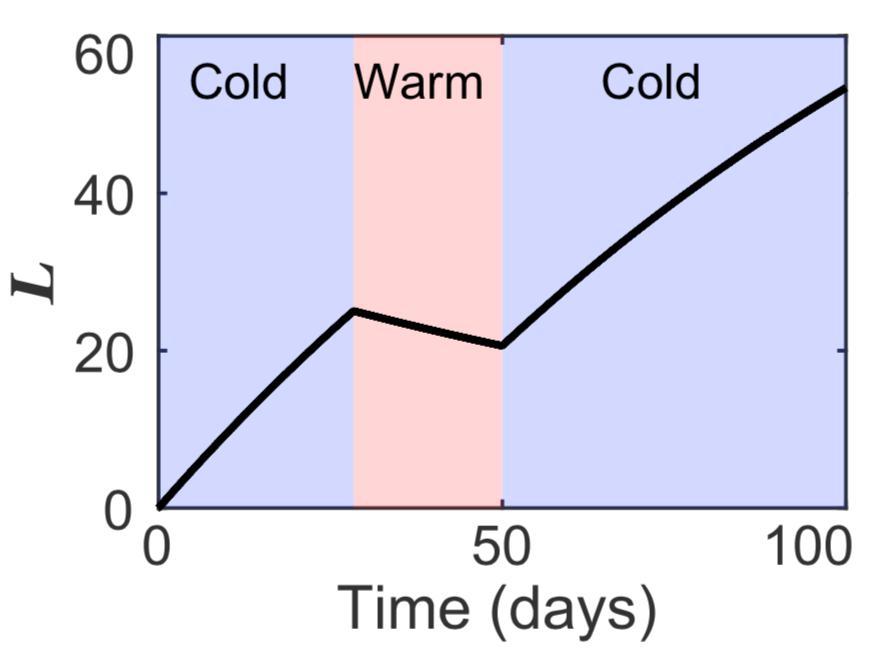
\includegraphics[width=1.0\textwidth]{./images/param_L.png}
    \end{minipage}
    \hfill
    \begin{minipage}{0.4\textwidth}
        \centering
        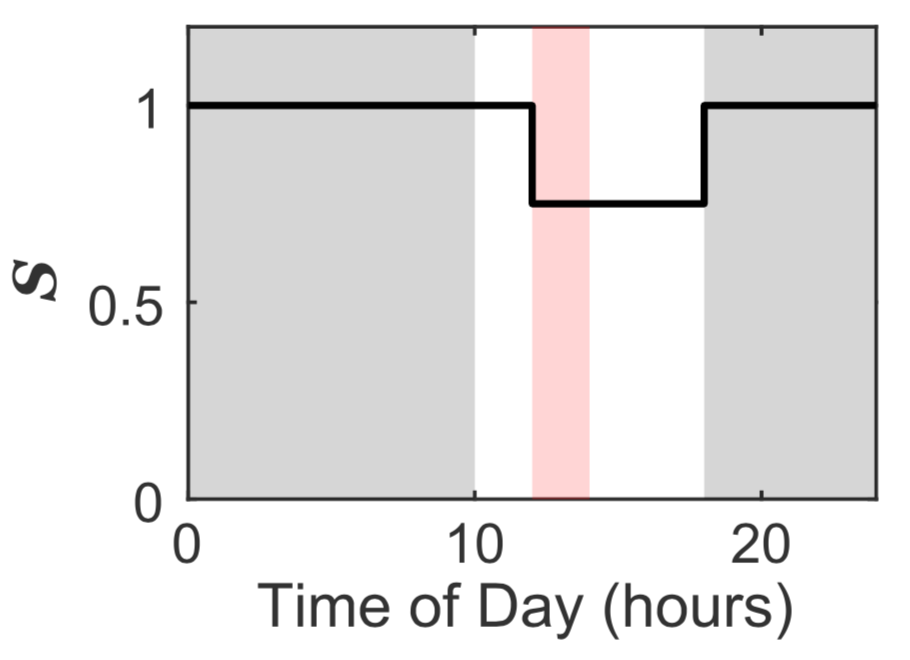
\includegraphics[width=1.0\textwidth]{./images/param_S.png}
    \end{minipage}
\end{figure}
\begin{figure}[h!]
    \centering
    \begin{minipage}{0.4\textwidth}
        \centering
        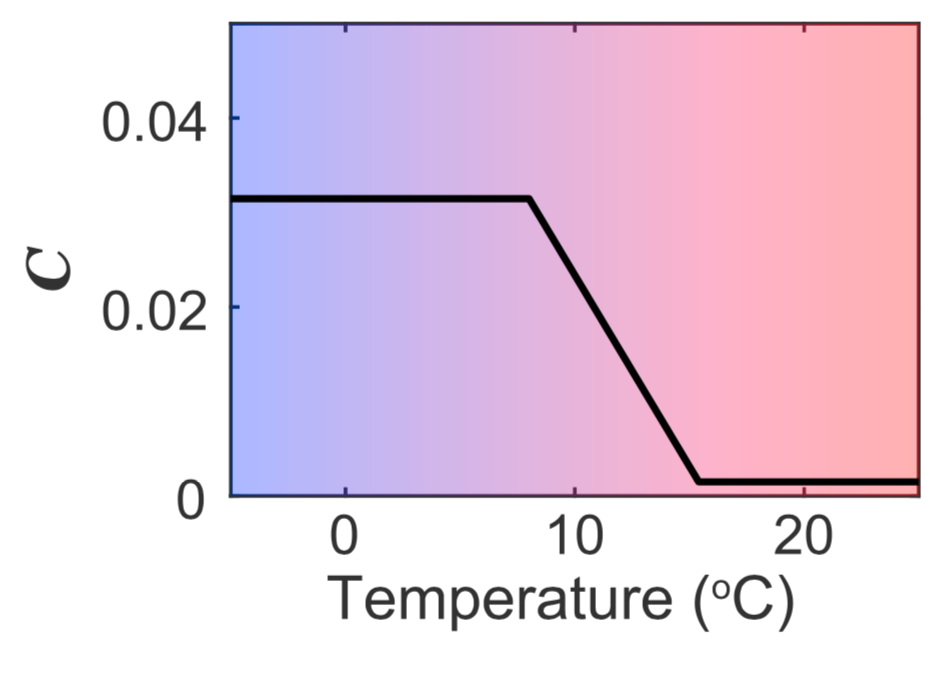
\includegraphics[width=1.0\textwidth]{./images/param_C.png}
    \end{minipage}
    \hfill
    \begin{minipage}{0.4\textwidth}
        \centering
        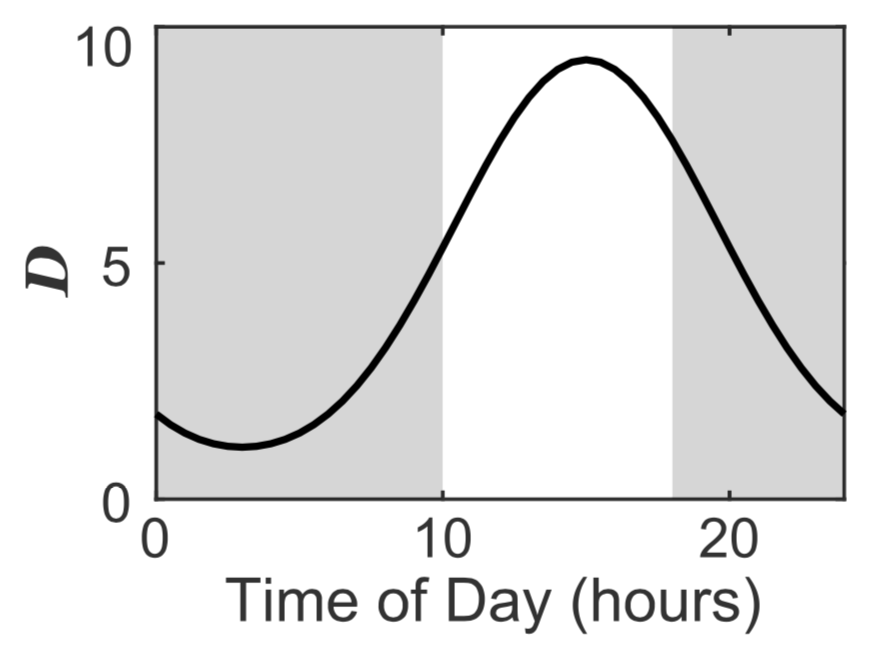
\includegraphics[width=1.0\textwidth]{./images/param_D.png}
    \end{minipage}
\end{figure}

\newpage
\begin{figure}[h!]
    \centering
    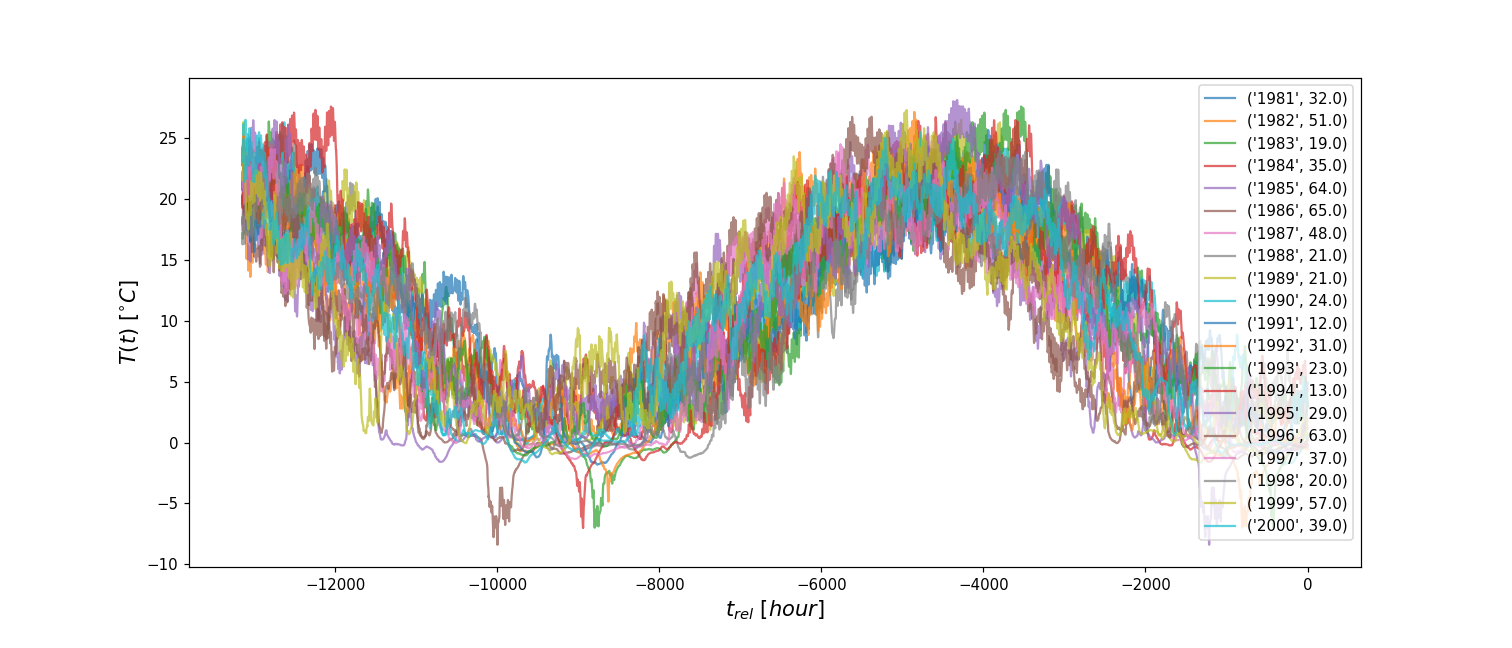
\includegraphics[width=0.75\textwidth]{images/temp_plot.png}
\end{figure}

\begin{figure}[h!]
    \centering
    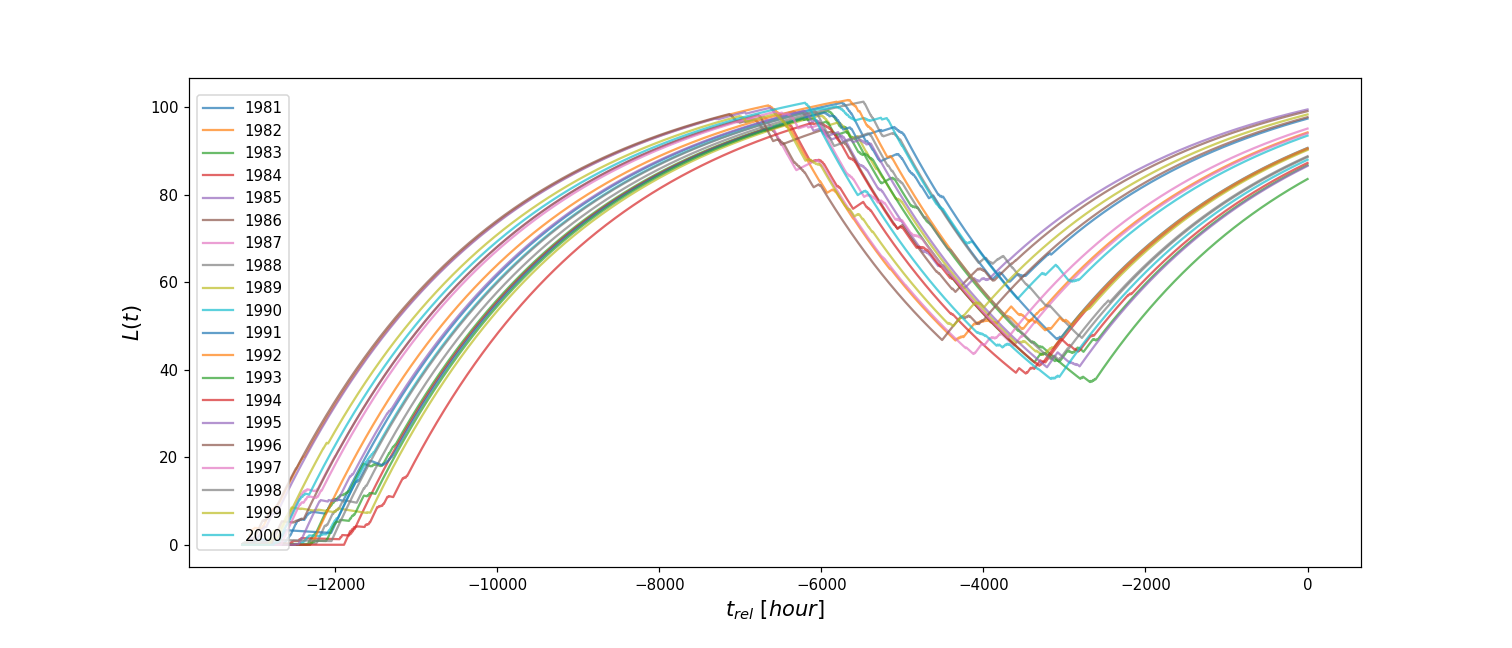
\includegraphics[width=0.75\textwidth]{images/L_plot.png}
\end{figure}

\newpage
\begin{figure}[h!]
    \centering
    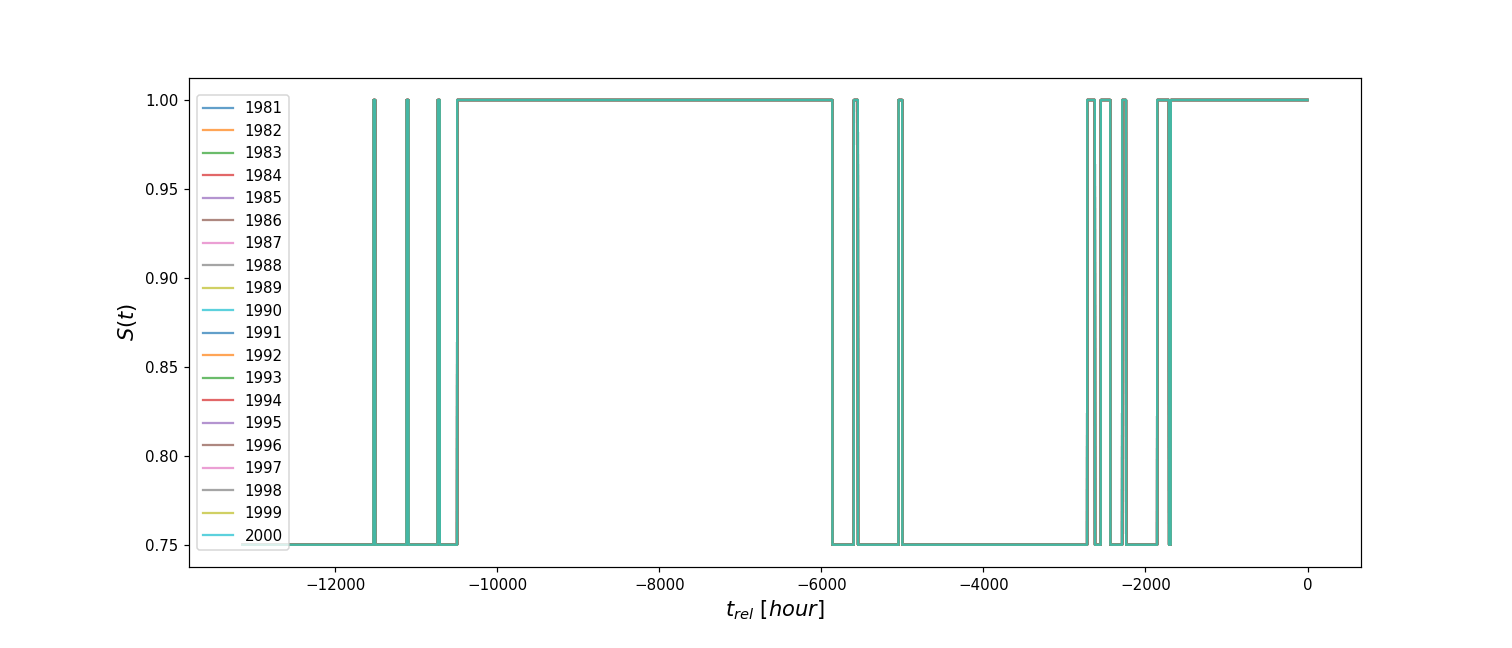
\includegraphics[width=0.75\textwidth]{images/S_plot.png}
\end{figure}
\begin{figure}[h!]
    \centering
    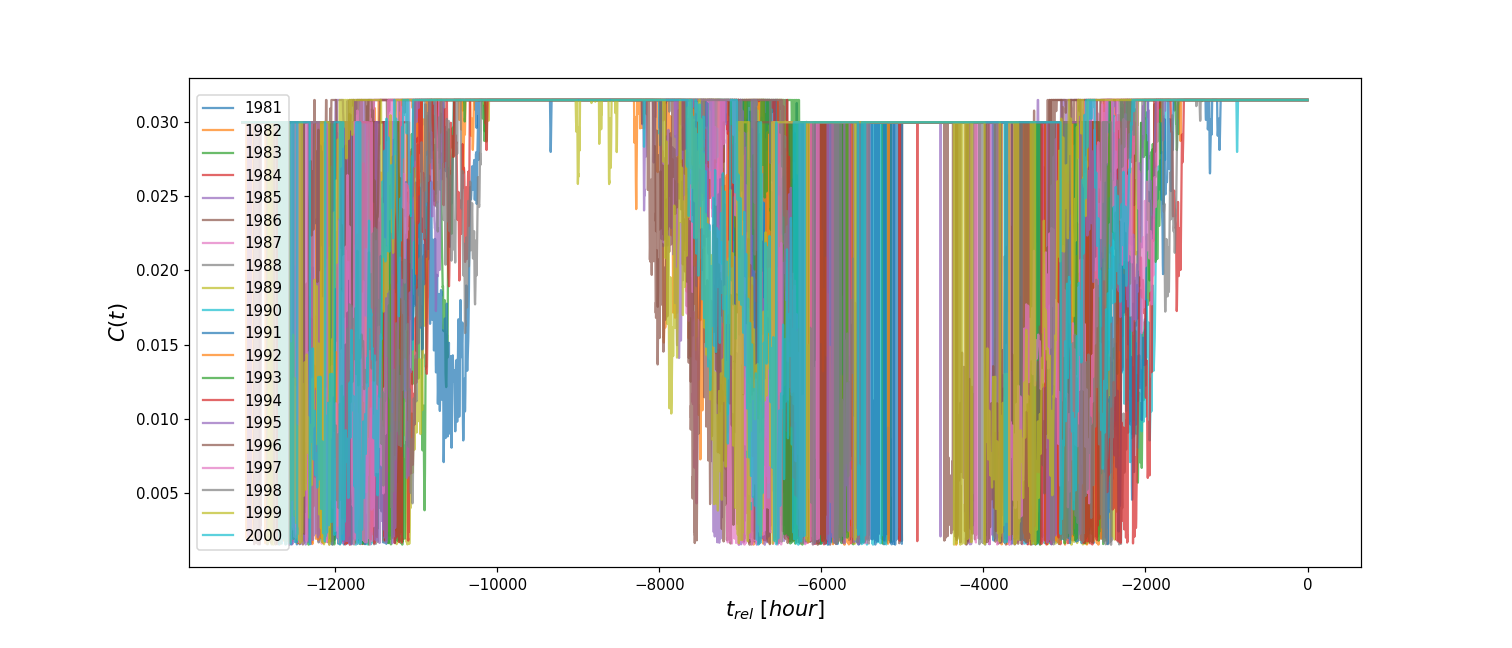
\includegraphics[width=0.75\textwidth]{images/C_plot.png}
\end{figure}
\begin{figure}[h!]
    \centering
    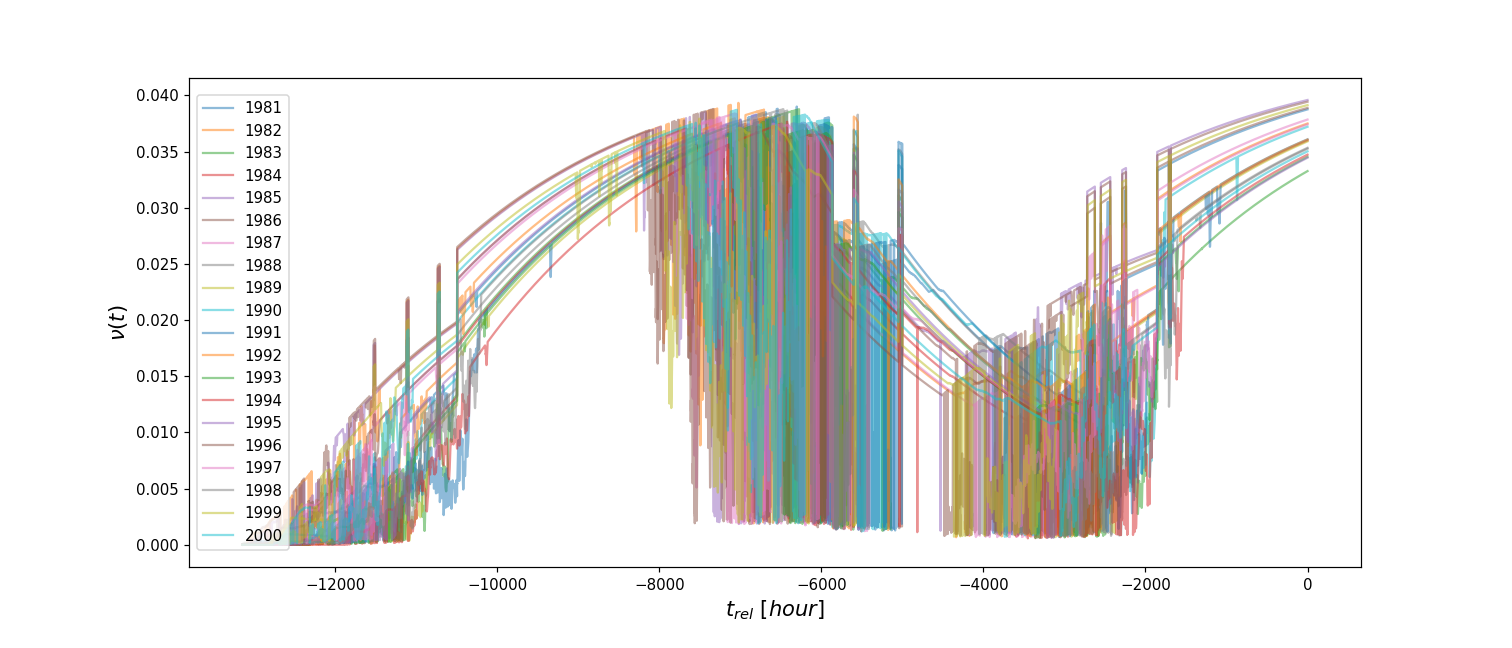
\includegraphics[width=0.75\textwidth]{images/nu_plot.png}
\end{figure}

\feynmandiagram [horizontal=a to b]{
    i1 -- [fermion] a -- [fermion] i2, a -- [photon] b,
    f1 -- [fermion] b -- [fermion] f2,
};

\begin{equation}
    \feynmandiagram [baseline=(d.base), horizontal=d to b] {
        a -- [fermion] b -- [fermion] c,
        b -- [boson] d [particle=\(\gamma\)], 
    };
    = i g_{e} \gamma^{\mu}
\end{equation}

\begin{equation}
    \feynmandiagram [inline=(d.base), horizontal=d to b] {
        a -- [fermion] b -- [fermion] c,
        b -- [boson] d [particle=\(\gamma\)],
    };
    = i g_{e} \gamma^{\mu}
\end{equation}

 % No invisible to keep the two photons together
 \feynmandiagram [small, horizontal=a to t1] {
    a [particle=\(\pi^{0}\)] -- [scalar] t1 -- t2 -- t3 -- t1, t2 -- [photon] p1 [particle=\(\gamma\)],
    t3 -- [photon] p2 [particle=\(\gamma\)],
};
\end{document}